% !TeX root = ../apuntes-ea.tex

\chapter{El teorema de Cauchy}

\section{Consideraciones previas}

\subsection{Conjugación}

Cuando introdujimos los homomorfismos de grupos hicimos especial hincapié en un automorfismo al que llamábamos $\phi_g$ o $\gamma_g$ y que para un $g \in G$ dado se definía como
\begin{align*}
	\phi_g : G &\to G\\
			x &\mapsto gx\inv{g}
\end{align*}

Diremos a partir de ahora que dos elementos son conjugados si cumplen la siguiente definición.

\begin{dfn}[Conjugados]
	\label{dfn:elementosconjugados}
	Sea $G$ un grupo, $a,b \in G$. Diremos que $b$ es conjugado de $a \iff \exists g \in G \mid b = ga\inv{g}$, es decir, si existe un $g\in G$ para el que el automorfismo conjugación $\phi_g$ cumple $\phi_g(a) = b$.
\end{dfn}

Observemos que la conjugación es una relación de equivalencia.

\begin{pro}
	Sea $R$ una relación de equivalencia definida con
	\begin{align*}
		\forall a,b \in G,\quad aRb \iff \exists g \in G \mid b = ga\inv{g}
	\end{align*}
\end{pro}

Probamos las tres propiedades de las relaciones de equivalencia:
\begin{enumerate}
	\item Reflexiva: $\forall a \in G,\ aRa$
	\begin{proof}
		Tomando $g = e$ se tiene $\forall a, a = ea\inv{e} = eae = a$.
	\end{proof}
	\item Simétrica: $\forall a,b \in G,\ aRb \iff bRa$
	\begin{proof}
		Se verifica la doble implicación tomando $g' = \inv{g}$ utilizado en el otro lado:
		\begin{align*}
			aRb \implies \exists g \mid b = ga\inv{g} \iff \inv{g}bg = a \iff g' = \inv{g} \land a = gb\inv{g} \iff bRa
		\end{align*}
		Hacia el otro lado es igual.
	\end{proof}
	\item Transitiva: $\forall a,b,c \in G,\ aRb \land bRc \implies aRc$
	\begin{proof}
		\begin{align*}
		aRb \implies \exists g_1 \mid b = g_1a\inv{g_1} \qquad\land \qquad bRc \implies \exists g_2 \mid c = g_2b\inv{g_2} \\
		c = g_2b\inv{g_2} = g_2g_1a\inv{g_1}\inv{g_2} \implies c = g'a\inv{g'} \text{ con } g' = g_1 g_2 \implies aRc
		\end{align*}
	\end{proof}
\end{enumerate}

\textbf{Nota:} La relación de conjugación solo merece la pena en grupos no abelianos, porque en un grupo abeliano, cualquier par de elementos es conjugado.

\begin{ej}
	En $S_3$ afirmamos lo siguiente:
	\begin{itemize}
		\item que $1$ solo tiene como conjugado a sí mismo,
		\item que $\{(12),(13),(23)\}$ son conjugados entre sí,
		\item y que $\{(123),(132)\}$ también son conjugados entre sí.
	\end{itemize}
	Es decir, que la conjugación nos genera una partición con 3 cajas disjuntas.
\end{ej}

En esta relación de equivalencia, las clases de equivalencia son de la forma $cl(a) = \{ga\inv{g} \mid g \in G\}$ (conjuntos de los elementos que son conjugados de $a$). Queremos saber cuántos elementos hay en cada clase de equivalencia. Para ello introduciremos la noción de centralizador de un elemento y posteriormente daremos un teorema (\autoref{pro:cardinalcajas}) que relaciona el número de elementos del centralizador de un elemento con el número de elementos de la clase de equivalencia de un elemento.

%TODO: definición de clase de equivalencia por la relación de conjugación?


\subsection{Centro de un grupo}

\begin{dfn}[Centro de un grupo]
	\label{dfn:centro}
	Sea $G$ un grupo finito. Definimos el centro de $G$, $Z(G) = \{a \in G \mid \forall g \in G,\ ag = ga\}$.
\end{dfn}

El centro es útil en grupos finitos no abelianos ya que, en grupos abelianos, el centro es todo el grupo como veremos en la 
\autoref{pro:centroigualabeliano}.

\begin{pro}
	\label{pro:centrocerrado}
	Sean $a, b \in Z(G)$. Entonces $ab \in Z(G)$.
\end{pro}

\begin{proof}
	Tenemos que $ag = ga$ y que $bg = gb$. Ahora tenemos que probar que $g(ab) = (ab)g$. Es trivial manipulando $(ab)g = agb = gab$.
\end{proof}

\begin{pro}
	\label{pro:centronormal}
	Sea $G$ un grupo. $Z(G)$ es un subgrupo y además es un subgrupo normal.
\end{pro}

\begin{proof}
	Es un subgrupo porque es cerrado (ver \autoref{pro:centrocerrado}), contiene siempre al neutro (el centro conmuta con todos) y para todo $a \in Z(G)$, se tiene que $\forall b \in G,\ ab = ba \iff ab\inv{a} = b \iff b\inv{a} = \inv{a}b \iff \inv{a} \in Z(G)$.
	
	Es normal porque $\forall g \in G,\ Z(G)g = \{ag \mid a \in G \land \forall b \in G,\ ab = ba\} = \{ga \mid a \in G \land \forall b \in G,\ ab = ba\} = gZ(G)$.
\end{proof}

\begin{pro}
	\label{pro:subcentronormal}
	Si $H < Z(G)$ entonces $H$ es abeliano y normal.
\end{pro}

\begin{proof}
	Es abeliano porque $\forall g,g' \in Z(G),\ gg' = g'g$ y en particular esto se cumple para $g,g' \in G < G$.
	
	Es normal porque $\forall g \in G, gH = \{ga \mid a \in H \land \forall b \in G,\ gb = bg\} = \{ag \mid a \in G \land \forall b \in G,\ bg = gb\} = Hg$.
\end{proof}

\begin{pro}
	Sea $g \in G,\ \phi_g: G \to G$ el isomorfismo definido por $\phi_g(x) = gx\inv{g}$. Entonces
	\begin{align*}
	x \in Z(G) &\iff \forall g \in G, gx = xg \iff gx\inv{g} = x \\
	x \in Z(G) &\iff \forall g \in G,\ \phi_g(x) = x 
	\end{align*}
\end{pro}

\begin{pro}
	\label{pro:centroigualabeliano}
	$G$ es abeliano $\iff G = Z(G)$
\end{pro}

\begin{proof}
	Sea $a \in G \land o(a) = n$. Si $a$ es el único elemento de orden $n$ entonces $n = 2 \land a \in Z(G)$. Probamos primero que $n=2$. Si $a$ es el único elemento de orden $n$ entonces tiene que ocurrir que $a$ y $a^{n-1}$ tienen el mismo orden por lo que $1 = n-1 \implies n = 2$.
\end{proof}

La siguiente proposición es crucial para sacar conclusiones sobre los grupos sabiendo sobre sus órdenes y su centro.

\begin{pro}
	\label{pro:triplecentro}
	Si $G/Z(G)$ es cíclico de orden $n$ entonces $n = 1$. Otra manera de formularlo: Si $G/Z(G)$ es cíclico, entonces $G = Z(G)$. Otra manera más de formularlo: si $G/Z(G)$ es cíclico entonces $G$ es abeliano.
\end{pro}

\begin{proof}
	Supongamos que $G/Z(G) \isom \ZnZ$. Vamos a probar que $n$ tiene que ser 1. Supongmos que $G/Z(G) = \{\overline{\alpha_i}, i = 1, \dots, n\}$ donde $\overline{\alpha_i} = \alpha^i Z(G)$. Fijamos $g \in G$ con $g = \alpha^j h,\ h \in Z(G),\ 0 \leq j < n$ y fijamos $f' \in G$ con $g' = {\alpha^j}' h',\ h' \in Z(G),\ 0 \leq j' < n$. Entonces $gg' = \alpha^j h{\alpha^j}' h' = \alpha^{j+j'}hh' = {\alpha^j}' h' \alpha^j h = gg'$ (podemos conmutar las $h$ con cualquier elemento porque $h \in Z(G)$, por el contrario, los $\alpha$ no necesitamos conmutarlos, solo agruparlos cuando están juntos). Es decir, que $\forall g, g' \in G$ tenemos que $gg' = g'g$ por lo que $G$ es abeliano.
\end{proof}

\subsection{Centralizador de un elemento.}

\begin{dfn}[Centralizador de un elemento]
	\label{dfn:centralizador}
	Sea $a \in G$. Llamamos centralizador de $a$ al conjunto
	\begin{align}
	C(a) = \{g \in G \mid \gamma_g(a) = g a \inv{g} = a\}
	\end{align}
	Se tiene que $\forall a \in G,\ e \in C(a)$, es decir que $C(a)$ no es vacío.
\end{dfn}

\begin{pro}
	$a \in Z(G) \iff C(a) = G \iff [G:C(a)] = 1$
\end{pro}

\begin{proof}
	Es cristalina de las definiciones.
\end{proof}

\begin{pro}
	$C(a)$ es un subgrupo de $G$
\end{pro}

\begin{proof}
	Por el teorema \ref{thm:subconjuntocerrado} solo necesitamos probar la clausura, es decir, tenemos que probar que $\forall g,g' \in G,\ g \in C(a) \land g' \in C(a) \implies gg' \in C(a)$. Sale solo $(gg')a\inv{gg'} = gg'a\inv{(g')}\inv{g} = ga\inv{g} = a \in C(a)$.
\end{proof}

\begin{pro}
	\label{pro:cardinalcajas}
	$|cl(a)| = |\{ga\inv{g} \mid g \in G\}| = [G:C(a)]$ (el número de elementos de una clase de equivalencia es el índice del centralizador de un representante)
\end{pro}

De la proposición anterior se deduce que

\begin{cor}
	$|C(a)| = [G:cl(a)]$
\end{cor}

La prueba de la proposición se ve clara después de ver la prueba del teorema de Cauchy, así que la dejamos para después.


\section{Teorema de Cauchy}

\begin{thm}[de Cauchy]
	\label{thm:cauchy}
	Sea $G$ un grupo finito con $|G| = n$. Si $p$ es primo y $p\divides n$ entonces $G$ contiene un elemento de orden $p$.
\end{thm}

\begin{proof}
	Procedemos por casos:
	\begin{itemize}
		\item Si $G$ es abeliano. Descomponemos $|G| = n = p_1^{\alpha_1}p_2^{\alpha_2}\dots p_s^{\alpha_s}$. Por el teorema \ref{thm:noprobado1}, $G \isom \Z/p_1^{\beta_1}\Z \times \Z/p_2^{\beta_2}\Z \times \dots \times \Z/p_s^{\beta_r}\Z$ donde cada $\alpha_i$ es la suma de algunos $\beta_r \qed$.
		
		\item Si $G$ no es abeliano. Particionamos $G$ con la relación de equivalencia dada anteriormente (definición \ref{dfn:elementosconjugados}), $aRb \iff \exists g \in G \mid ga\inv{g} = b$. Recordemos que cada clase de equivalencia es de la forma $\overline{c} = \{gc\inv{g} \mid g \in G\}$. Observamos que si partimos de $e$, el elemento neutro, $eRb \implies \exists g \mid ge\inv{g} = b$ pero $\forall g \in G,\ ge\inv{g} = e$ por lo que $cl(e)$ tiene un único elemento.
		
		Tomemos ahora una clase de equivalencia, la que contenga a $a \in G$. La clase es $cl(a) = \{ga\inv{g} \mid g \in G\}$. Es claro que $a \in \overline{a}$ por la propiedad reflexiva de $R$, luego por lo menos en $cl(a)$ tiene un elemento.
		
		\begin{align*}
		cl(a) = \{ga\inv{g} \mid g \in G\} = \{a\} &\iff ga\inv{g} = a,\ \forall g \in G \\
		&\iff ga = ag,\ \forall g \in G
		\end{align*}
		\begin{align*}
		|cl(a)| = 1 &\iff \overline{a} = 1 \\
		&\iff a \in Z(G)
		\end{align*}
		
		Supongamos que la partición está dada por subconjuntos $cl(a_1), cl(a_2), \dots, cl(a_s)$. Por ser una partición, cualquier elemento vive en una sola caja, luego para saber cuantos elementos tiene $G$ nos vale con sumar los elementos de cada caja:
		\begin{align*}
		|G| = \sum_{i = 1}^{s} |cl(a_i)| = \sum_{i = 1}^n |\{ga_i\inv{g} \mid g \in G\}|
		\end{align*}
		Ahora bien, por la proposición \ref{pro:cardinalcajas} tenemos que $|cl(a_i)| = [G:C(a_i)]$. Por tanto decir que $|cl(a_i)| = 1 \implies [G:C(a_i)] = 1 \implies G = C(a_i)$.
		
		Ahora vamos a dividir el sumatorio en dos: por un lado las cajas de un solo elemento y luego las cajas de varios elementos:
		\begin{align}
		\label{eq:thmcauchy}
		|G| = |Z(G)| + \sum_{i = r + 1}^{s} [G : C(a_i)] \text{ donde } |Z(G)| = r \text{ y } [G : C(a_i)] \geq 2, \forall i = r+1,\dots, s
		\end{align}
		
		Ahora para probar el teorema de Cauchy procedemos por inducción en $n = |G| = [G:C(a_i)]\cdot |C(a_i)|$.
		
		\begin{enumerate}
			\item Caso $n = 1$. $G = \{e\}$ que es obvio.
			\item Caso $n = 2$. Son grupos cíclicos por lo que $\exists \alpha \in G \mid o(\alpha) = 2$.
			\item Caso $n \implies n+1$. Pueden pasar dos cosas:
			\begin{itemize}
				\item o bien $p \divides |C(a_i)|$ para algún $i = r+1, \dots, s$ entonces, por hipótesis inductiva, $C(a_i)$ contiene algún elemento de orden $p$. Pues ya está: $C(a_i) < G$ porque $\alpha \in C(a_i) \mid o(\alpha) = p \implies \alpha \in G$ también). \qedsymbol
				
				\item o bien $p \not\divides |C(a_i)|,\ \forall i = r+1,\dots,s$. No podemos proceder por inducción. Por hipótesis $|G| = [G:C(a_i)]\cdot |C(a_i)| \land p \divides |G| \implies p \divides [G: C(a_i)],\ \forall i = r+1,\dots, s$.
				
				Como $|G| = |Z(G)| + \sum_{i = r + 1}^{s} [G : C(a_i)]$ y por hipótesis $p \divides |G| \land p \divides [G : C(a_i)], \forall i = r+1,\dots,s \implies p \divides |Z(G)| \implies |Z(G)|$ es múltiplo de $p$. Como $Z(G)$ es abeliano, $\exists \alpha \in Z(G) \mid o(\alpha) = p$. Luego se reduce al caso abeliano y ya estaría \qedhere
			\end{itemize}
		\end{enumerate}
	\end{itemize}
\end{proof}

\begin{ej}
	Sea $G$ tal que $|G| = pq$. Entonces por le teorema de Cauchy $\exists a,b \in G \mid o(a) = p \land o(b) = q$. Como $p$ y $q$ son primos los ordenes de $\langle a \rangle$ y $\langle b \rangle$ son coprimos y por tanto $\langle a \rangle \cap \langle b \rangle = \{e\}$. Por el teorema del orden de conjunto producto libre (\ref{thm:cardinalidadproductolibre}), $|\gen{a} \gen{b}| = pq$. No sabemos si se tendrá que $G = \gen{a}\gen{b}$ ya que al no saber si alguno es normal, no podemos afirmar que el producto libre sea un grupo. Lo que si que sabemos es que $G = \{a^ib^j \mid 0 \leq i < p -1 \land 0 \leq j < q - 1\} = \langle a, b \rangle$.
\end{ej}

\begin{ej}
	Sea $G$ tal que $|G| = 2q$. Análogamente al caso anterior llegamos a que $o(a) = 2$. Como $\langle b \rangle$ tiene índice 2 entonces $\langle b \rangle \normsub G$. Esto nos permite saber como operar con las palabras $a^ib^j$ una vez tenemos un isomorfismo que lleva $a b \inv{a} = b^j$ (tiene que ir a algún $b^j$ porque por ser isomorfismo tiene que llevar elementos de orden $q$ en elementos de orden $q$: los $b \in \langle b \rangle$)
\end{ej}

Dada la relación de equivalencia de conjugación (definición \ref{dfn:elementosconjugados}), definimos $C$ como el conjunto de los representantes de las clases de equivalencia. Entonces podemos decir
\begin{align*}
G = \bigcup_{c_i \in C} \{a \in G \mid a R c_i\}
\end{align*}
Observemos que $d \in Z(G) \iff \{a \in G \mid a R d\} = \{gd\inv{g} \mid g \in G\} = \{d\}$. Y por tanto podemos escribir
\begin{align*}
C = Z(G) \cup (C\setminus Z(G))
\end{align*}
que aunque pareza obvio quiere decir que $C$ se puede expresar como la unión disjunta de las cajas que tienen solo un elemento que se corresponden con elementos que están en el centro y las cajas que tienen más de uno. Y por lo visto en la demostración del teorema de Cauchy tenemos que
\begin{align*}
|G| = \sum_{c_i \in C} | \overline{c_i} | = |Z(G)| + \sum_{i = r + 1}^{s} [G : C(a_i)] \text{ donde } [G : C(a_i)] \geq 2
\end{align*}

\subsection{P-grupos}

Una aplicación inmediata del teorema de Cauchy es la caracterización de los $p$-grupos.

\begin{dfn}[P-grupo]
	Sea $p$ primo. Decimos que $G$ es un p-grupo si $|G| = p^r$.
\end{dfn}

\begin{thm}
	Si $G$ es un p-grupo entonces $Z(G)$ es no trivial (no es el vacío).
\end{thm}

\begin{proof}
	Podemos escribir sin distinguir entre cajas de uno o varios elementos
	\begin{align*}
	|G| = |C(c_i)||[G:C(c_i)]|
	\end{align*}
	es decir que tenemos una factorización de $|G| = p^r$ luego $|C(c_i)|$ y $|[G:C(c_i)]|$ son ambos potencias de $p$. Y aplicando esto a la expresión \ref{eq:thmcauchy} tenemos que
	\begin{align*}
	\underbrace{|G|}_{\text{múltiplo de p}} = |Z(G)| + \sum_{i = r + 1}^{s} \underbrace{[G : C(a_i)]}_{\text{múltiplo de p}} \text{ donde } [G : C(a_i)] \geq 2
	\end{align*}
	por lo que $|Z(g)|$ tiene que ser múltiplo $p$ por lo que $Z(G)$ no puede ser el trivial.
\end{proof}

Véase un ejemplo de aplicación de esta anterior proposición en el ejercicio \nameref{ex:h2.22} y en el ejercicio \nameref{ex:h1.33}

\begin{ej}
	Tenemos que $Z(D_4) = \{1,B^2\}$ y $Z(H) = \{1, B^2\}$ donde $H$ es el grupo de cuateriones (\autoref{ej:grupocuaterniones}) y $D_4$ es el famoso grupo (\autoref{ej:famosogrupod4}).
\end{ej}

\begin{pro}
	\label{pro:primocuadradoabeliano}
	Si $p$ es primo y $|G| = p^2$ entonces $G$ es abeliano.
\end{pro}

\begin{proof}
	Por el la demostración del teorema anterior tenemos que o bien $|Z(G)| = p$ o bien $|Z(G)| = p^2$. Afirmamos que $|Z(G)| \neq p$ ya que si fuera así $|G/Z(G)| = p \implies G/Z(G)$ cíclico pero hemos probado (proposición \ref{pro:triplecentro}) que $G/Z(G)$ no puede ser cíclico. Por lo tanto $|Z(G)| = p^2 \implies Z(G) = G \implies G$ es abeliano.
\end{proof}


\section{Más sobre la conjugación, el centro y los centralizadores.}
Antes de introducir el teorema de Cauchy hablábamos de la conjugación que era una relación de equivalencia que partía un grupo $G$ en cajas. Nos gustaría saber cuántos elementos había en la clase de equivalencia de cada uno de los elementos de $G$ y para eso introducíamos el concepto de centralizador de un elemento: $C(a)$ el conjunto de los elementos de $G$ que no mueven a $a$ por conjugación. La \autoref{pro:cardinalcajas} nos aseguraba que $|cl(a)| = [G:C(a)]$ y dijimos que retrasaríamos la prueba hasta ahora. Pues aquí va.



Sea $\sim$ una relación de equivalencia definida por $a\sim b \iff \exists g \in G \mid ga\inv{g} = b$ para $a,b \in G$. Esta relación da una partición de $G$ en clases de la forma $cl(a) = \{ga\inv{g} \mid g \in G\}$. En el caso abeliano esta relación es la de igualdad, por lo que no nos merece la pena liar este pifostio para saber que $a\sim b \iff a = b$. 

Es muy importante saber cómo contamos los elementos de una clase, es decir, de cuantas formas podemos \textit{mover} el elemento $a$ con $g \in G$. Para ello definimos el centralizador (definición \ref{dfn:centralizador}) como $C(a) = \{h \in G \mid ha\inv{h} = a\} < G$. Queremos probar que $|cl(a)| = [G:C(a)] = r$.

\begin{proof}[Demostración de la \autoref{pro:cardinalcajas}]
	
	Lo probamos tomando clases laterales a la izquierda (por ejemplo) y partiendo $G$ en $r$ cajas. Las cajas son de la forma $\alpha_iC(a),\ i = 1, \dots, r$. Esta partición no tiene que ver con la partición anterior. Observemos que para cualquier $g \in \alpha_i C(a), g = \alpha_i h$, tenemos que $g a \inv{g} = \alpha_i h a \inv{h} \inv{\alpha_i} = \alpha_i a \inv{\alpha_i}$ es decir que los $g \in C(a)$ no se mueven fuera de la caja. Es decir, que si $\alpha_i \neq \alpha_j$ para $i\neq j$ entonces hay $r$ maneras de mover a $g$ y por tanto $|cl(a)| = r$.
	
	Probaremos que en efecto los $\alpha_i$ son distintos.
	
	Sean $g_1, g_2 \in G$. $g_1a\inv{g_1} = g_2a\inv{g_2} \iff (\inv{g_2}g_1)a(\inv{g_1}g_2) = a \iff (\inv{g_2}g_1)a\inv{(\inv{g_2}g_1)} \iff C(a) \inv{g_2}g_1 \in C(a) \iff g_1 \in g_2C(a)$.
	
	Si $G/\sim$ tiene $N$ elementos, tomamos $\{c_1, \dots, c_N\}$ como el conjunto de los representantes, donde $c_i$ es un representante de cada conjunto de la partición. Entonces pordemos expresar
	\begin{align*}
	G = \bigcup_{c_i \in C} = cl(c_i)
	\end{align*}
	donde $|cl(c_i)| = [G:C(c_i)]$. Por tanto decir que $|cl(c_i)| = 1$ es equivalente ($\iff$) a decir que $G = C(c_i) = \{\forall g \in G,\ gc\inv{g} = c\} \iff c \in Z(G)$.
	
	Afirmábamos que
	\begin{align*}
	|G| = \sum_{c_i \in C} |cl(c_i)| = |Z(G)| + \sum_{c_i \in C\setminus Z(G)} [G:C(c_i)]
	\end{align*}
	descomponiendo la suma en las clases con solo un elemento y las clases con más de dos elementos.
\end{proof}



\begin{ej}
	Consideramos $D_3$ (ver \autoref{ej:diedricosordengenerico}). Nos fijamos en que $B \not\in Z(D_3)$ es decir que en $cl(B)$ hay más de un elemento. En particular por lo visto anteriormente $|cl(B)| = [G:C(B)]$. Ahora bien $C(B) = \{1, B, B^2\}$ luego $|cl(B)| = [G:C(B)] = 2$. La pregunta es ¿quién es el compañero de $B$ en su clase? Es fácil, recordamos que $\phi_g (x) = gx\inv{g}$ (el isomorfismo conjugación) es un isomorfismo y que $\{1, B, B^2\}$ es normal, por lo que $o(B) = o(\phi_g(B)) = 2$. Entonces $\phi_g(B) \neq 1$ porque no coinciden los órdenes, de manera que $\phi_g(B) = B^2$ por necesidad. Luego el otro elemento es el $B^2$.
	
	¿Qué pasa con el elemento $A$? Pues ocurre que $A \in C(A)$ y $\{1, A\} \in C(A)$ y en realidad no puede haber más porque si hubiese un tercero, $\{1, A\}$ es un subgrupo de orden 2 $\implies o(\{1, A\})$ no divide a 3 $\implies$ si hubiese más, $C(A) = D_3$ y eso no puede ser $\implies C(A) = \{1, A\} \implies |cl(A)| = [D_3:C(A)] = 6/2 = 3$. Como las clases son disjuntas los tres elementos sobrantes forman la última caja.   
	
	Para conlcuir queda que la relación $\sim$ parte $D_3$ en 3 cajas, a saber:
	\begin{align*}
	D_3 = \{\underbrace{1}, \underbrace{B, B^2}, \underbrace{A, AB, AB^2}\}
	\end{align*}
\end{ej}


\begin{ej}
	\label{ej:clasesd4}
	El caso del famoso grupo $D_4$ (ver ejemplo \ref{ej:famosogrupod4})es mucho más interesante porque $Z(D_4)$ no es trivial. Elegimos por ejemplo el elemento $B^2$. Probar que $\phi_g(B^2) = gB^2\inv{g} = B^2,\ \forall g \in D_4$ es complicado. Pero fijémonos en que $\phi_B(B^2) = BB^2\inv{B} = B^2$ y que $\phi_A(B^2) = AB^2\inv{A} = B^2$. Entonces cualquier palabra en $A$ y en $B$ no mueve a $B^2$, por ejemplo $AB(B^2)\inv{B}\inv{A} = B^2$. Nos convencemos de que $B^2 \in Z(D_4)$. Con esto ya tenemos que $|Z(D_4)| \geq 2$ (puesto que de momento ya sabemos que $1, B^2 \in Z(G)$. Podría ser entonces $|Z(D_4)| = 4, 8$ (probamos los divisores de $|D_4|$). Como $D_4$ no es abeliano, es claro que $|Z(D_4) \neq 8$. Tampoco puede ser $|Z(D_4) \neq 4$ porque si tuviera 4, el cociente $D_4/Z(G)$ tendría orden $2$ y por tanto sería cíclico. Pero ya hemos probado que $G/Z(G)$ no puede ser cíclico (ver proposición \ref{pro:triplecentro}). Luego ya sabemos que $Z(D_4) = \{1, B^2\}$.
	
	Vamos a seguir sacando cajas. Veamos $cl(B)$. Claramente $B \in C(B)$ y por alguna razón que me falta $C(B) = \{1, B, B^2, B^3\}$. Por la fórmula tenemos que $|cl(B)| = [D_4:C(B)] = 2$. Tenemos una vez más que utilizar el isomorfismo de conjugación. Sabemos que $cl(B) = \{ga\inv{g} \mid g \in G\}$. Pero al ser $\phi_g$ isomorfismo y $\langle B \rangle$ normal, tenemos que $\phi_g : \langle b \rangle \to \langle b \rangle$ también es isomorfismo y por tanto lleva elementos de orden $n$ en elementos de orden $n$. Por tanto $\phi_g(B) = gB\inv{g}$ solo puede ser $B^3$ (a parte de $B$). Luego ya tenemos que $cl(B) = \{B, B^3\}$.
	
	¿Qué pasa con $A$? Pues es claro que $C(A) \supset \{1, A, B^2, AB^2\}$ ya que $B^2 \in Z(G)$ por lo que está en todos los $C(c_i)$.
	
	
	Segundo intento.
	
	\begin{enumerate}
		\item Como siempre $cl(e) = \{e\}$
		\item Veamos $cl(B)$. Queremos ver cuántos elementos tiene. Sabemos que $|cl(B)| = [D_4:C(B)]$. Veamos quién es $C(B)$. En primer lugar $B \in C(B) \implies \gen{B} \in C(B)$. Así ya tenemos que $|C(B)| \geq 4$. ¿Puede haber algún elemento más en $C(B)$? No, porque si hubiera uno más, su orden ya sería $|C(B)| = 8$ pues $C(B) < D_4$. Así concluímos que $|cl(B)| = [D_4:C(B)] = 8 / 4 = 2$. Además sabemos que $[D_4:C(B)] = 2 \implies C(B) \normsub D_4 \iff gC(B)\inv{g} = C(B) \forall g \in D_4 \implies gB\inv{g} \in C(B)$. Además como $gx\inv{g}$ es un isomorfismo que lleva elementos de orden $n$ en elementos de orden $n$ obtenemos que $o(gB\inv{g}) = o(B) = 2$. Sabemos que $B \in cl(B) \land cl(B) = \{gB\inv{g} \mid g \in D_4\} \land gB\inv{g} \in C(B) \implies gB\inv{g} = B^3$. Por tanto $cl(B) = \{B, B^3\}$.
		\item Veamos $cl(A)$. Queremos ver cuántos elementos tiene. Sabemos que $|cl(A)| = [D_4:C(A)]$. Veamos quién es $C(A)$. En primer lugar $A \in C(A) \implies \gen{A} \subset C(A)$. Si $B \in C(A)$ entonces $C(A) = G$ pues $B$ y $A$ generan. Esto no puede ser porque $C(A) = G \implies A$ conjuga con todos los demás elementos pero sabemos que $AB \neq BA$. Ocurre lo mismo con $B^3$. Probamos con $B^2$. $B^2AB^2 = BBAB^2 = BAB^3B^2 = BAB = AB^3B = A$ luego $B^2 \in C(A)$. Como $C(A) < D_4$ sabemos que es cerrado y por tanto $AB^2 \in C(A)$. Ya no puede haber más elementos porque si hubiera más, entonces $|C(A)| = 8$ y eso no puede ser. Por tanto $|cl(A)| = [D_4:C(A)] = 8 / 4 = 2$. Sabemos que $A \in cl(A)$. ¿Quién es el otro elemento? Como antes, $[D_4:C(A)] = 2 \implies C(A) \normsub D_4 \iff gC(A)\inv{g} = A$. Como $gx\inv{g}$ es un isomorfismo mantiene el orden y por tanto los conjugados de $A$ pueden ser $B^2$ o $AB^2$ (los únicos de orden 2 en $C(A)$
	\end{enumerate}
\end{ej}

\section{Normalizador de un subconjunto}

Vez pasada tomábamos $a \in G$ y teníamos $cl(a) = \{g a \inv{g} \mid g \in G\} = \{a=a_1, a_2, \dots, a_r\}$ y $C(a) = \{g \in G \mid ha\inv{h} = a \}$. Concluíamos que $|cl(a)| = [G:C(a)]$.

Vamos a generalizar al caso $S \subset G,\ S \neq \emptyset$. Consideramos la familia de subconjuntos siguiente:
\begin{align*}
\{gS\inv{g} \mid g \in G\} = \{S = S_1, S_2, \dots, S_r\}
\end{align*}
que tiene $r$ subconjuntos distintos.

Recordemos que la conjugación dada $\phi_g(x) = gx\inv{g}$ (el isomorfismo conjugación) es un isomorfismo\footnote{A veces tomate frito llama a este isomorfismo $\gamma_g$}, y por tanto una biyección entre subconjuntos $S_i \subset G$. Por tanto $|S| = \phi_g(S)$.

\begin{dfn}[Normalizador de un subconjunto]
	\label{dfn:normalizador}
	Fijado $S \subset G$, definimos el normalizador de $S$:
	\begin{align}
	N(S) = \{g \in G \mid gS\inv{g} = S\}
	\end{align} 
\end{dfn}

Se parece mucho a la definición de centralizador de un elemento (\autoref{dfn:centralizador}). En el caso en que $S = \{a\}$ tenemos que $N(S) = \{g \in G \mid ga\inv{g} = a\} = C(a)$.

Ojo, decir que $gS\inv{g} = S$ no significa que $\forall b_i \in S,\ gb_i\inv{g} = b_i$, sino que $gb_i\inv{g} \in S$ (no mandamos cada elemento a él mismo, sino que todos quedan dentro del subconjunto). Es decir que \textit{$N(S)$ es el conjunto de la totalidad de elementos para los que $\phi_g$ manda el subconjunto $S$ en sí mismo.}

\begin{pro}
	Dado $S \subset G,\ N(S)$ es un subgrupo.
\end{pro}

\begin{proof} Como $G$ es finito, $N(S)$ es subgrupo $\iff S \neq \emptyset \land N(S)$ es cerrado por la operación.
	\begin{itemize}
		\item Es claro que $e \in N(S)$ pues $eS\inv{e} = S$, luego $N(S) \neq \emptyset$.
		\item Tenemos que probar la clausura. Si $h_1S\inv{h_1} = S \land h_2S\inv{h_2} = S$ tenemos que $\underbrace{(h_2S\inv{h_2})}_{\in S}\inv{h_1} = S \implies h_1h_2 \in N(S)$.
	\end{itemize}
\end{proof}

\begin{pro}
	\label{pro:propiedad2Ns}
	$\{gS\inv{g} \mid g \in G\} = \{S = S_1, S_2, \dots, S_r\}$ son $r$ subconjuntos distintos. Es decir que $r = [G: N(S)]$.
\end{pro}

\begin{proof}
	A la izquierda del lector.\footnote{Left to the reader.}
\end{proof}

Supongamos ahora que en vez de ser $S \subset G$, tomamos $S < G$. Recordemos que dado $g\in G$, $\phi_g$ es un isomorfismo por tanto manda elementos de un subgrupo en otro subgrupo (si el subgrupo es normal, manda elementos de un subgrupo en sí mismo). Es por esto que la afirmación equivalente a la proposición anterior sería:

\begin{pro}
	Sea $S < G$. Entonces $\{gS\inv{g} \mid g \in G\} = \{S = S_1, S_2, \dots, S_r\}$ son $r$ subgrupos distintos.
\end{pro}

% TODO aquí había un teorema (el 3 de la página 80 de santorum que no hay quien lo entienda)

\begin{thm}
	Sea $G$ grupo, $H < G$. Entonces $H \normsub N(H)$ y $N(H)$ es el mayor subgrupo de $G$ con esta propiedad, es decir, $H \normsub H' \implies H' < N(H)$.
\end{thm}

\begin{proof}$ $\newline
	\begin{itemize}
		\item Para probar que $N\normsub N(H)$ tiene sentido olivdarse del grupo $G$. Tenemos que $h \in N(H) \iff hH\inv{h} = H, \forall h \in G$. En particular, tenemos que $hH\inv{h} = H,\ \forall h \in N(H) \implies H$ es normal en $N(H)$.
		
		\item Para porbar que $N(H)$ es el mayor subgrupo con esta propiedad demostraremos que si $H < H'$ y $H \normsub H'$ entonces $H' \subseteq N(H)$. La demostración es casi una tautología. Tenemos que $\forall h' \in H',\ h'H\inv{h'} = H \implies \forall h' \in H',\ h' \in N(H) \implies H' \subset N(H)$.
	\end{itemize}
\end{proof}

\begin{cor}
	$H \normsub G \iff N(H) = G$
\end{cor}

\begin{proof}
	Sabemos que $H\normsub H = \{gH\inv{g} \mid g \in G\}$ y dicho conjunto tiene $[G:N(H)] = 1$ elementos, luego $N(H) = G$. En otras palabras, el normalizador de un subgrupo $H < G$ normal es todo el grupo $G$.
\end{proof}

\begin{pro}
	Si $H < G$ entonces\footnote{No sé si la hipotesis aquí es que $H < G$ o que $H \subset G$} $Z(G) < N(H)$
\end{pro}

\begin{proof}
	Por definición de $Z(G)$ tenemos que los elementos $g \in Z(G)$ fijan no solo los elementos dentro de subconjuntos, sino que los fijan uno a uno. Por lo que es claro que $Z(G) < N(H)$. 
\end{proof}

\begin{pro}
	\label{pro:centralizadorsubgruponormalizador}
	Sea $g \in G$. Entonces $C(g) < N(\gen{g})$
\end{pro}

\begin{ej}
	Vamos a empezar por $G = S_3$. En $S_3$ tenemos los subgrupos $\langle (12) \rangle, \langle (13) \rangle, \langle (23) \rangle$ de orden 2 y el subgrupo $\langle (123) \rangle = \{(1), (123), (132)\}$ de orden 3.
	
	\begin{figure}[h]
		\centering
		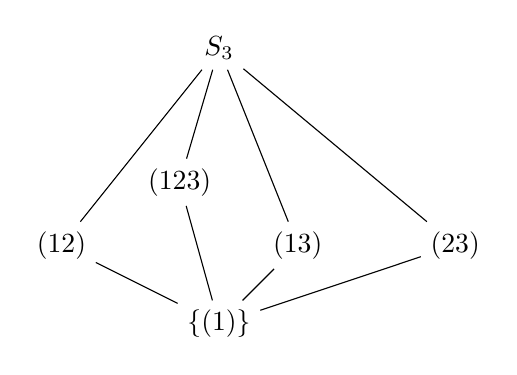
\begin{tikzpicture}
			\node (neut) at (0,0) {$\{(1)\}$};
			\node (12) at (-2,1) {$\gen{(12)}$};
			\node (13) at (1, 1) {$\gen{(13)}$};
			\node (23) at (3,1) {$\gen{(23)}$};
			\node (123) at (-0.5,1.8) {$\gen{(123)}$};
			\node (s3) at (0,3.5) {$S_3$};
			
			\draw (neut) -- (12) -- (s3);
			\draw (neut) -- (23) -- (s3);
			\draw (neut) -- (13) -- (s3);
			\draw (neut) -- (123) -- (s3);
		\end{tikzpicture}
		\caption{Retículo de subgrupos de $S_3$}
		\label{fig:reticulos3}
	\end{figure}
	\begin{itemize}
		\item En el caso de este último $g\langle (123) \rangle \inv{g} = \langle (123) \rangle$ porque es el único subgrupo de orden 3. Por tanto $\langle (123) \rangle \normsub S_3$ y entonces $N(\langle (123) \rangle) = S_3$.
		\item Sin encambio en el caso de los subgrupos de orden $2$ es posible que $g\langle (12) \rangle \neq \langle (12) \rangle$, porque hay más de un subgrupo de orden 2. Observemos por ejemplo que $(13)(12)\inv{(13)} = (32) = (23)$, luego $\langle (12) \rangle$ no es normal en $S_3$, ya que hemos encontrado $g = (13) \in G$ que lo mueve. Pero ¿quién es el normalizador $N(\langle (12) \rangle)$? Pues ya sabemos que es un subgrupo propio, porque no puede dar todo $S_3$. Evidentemente $\langle (12) \rangle \subset N(\langle (12) \rangle)$. Luego tiene que ser que $N(\langle (12) \rangle) = \langle (12) \rangle$\footnote{No tiene gracia que $\langle (12) \rangle$ sea normal en sí mismo, lo que tiene gracia es que $\langle (12) \rangle$ es el mayor grupo donde $\langle (12) \rangle$ es normal.} 
	\end{itemize}
\end{ej}

%20181011

\begin{ej}
	Seguimos por \nameref{ej:famosogrupod4}). Vimos anteriormente (\autoref{ej:clasesd4}) que $Z(D_4) = \{1, B^2\}$. Tenemos su retículo en \autoref{fig:reticuloD4}. Queremos ver de entre los subgrupos de $D_4$, cuáles son los que conmutan.
	\begin{itemize}
		\item Empecemos por $\langle B \rangle = \{1, B, B^2, B^3\}$. Observamos que $\langle b \rangle$ es normal puesto que tiene índice 2, es decir que $\{g\langle B \rangle \inv{g} \mid g \in G\} = \{\langle B \rangle\}$ y tiene sentido que $[G:N(\langle B \rangle)] = 1$. Es decir que como $\langle B \rangle$ es normal tenemos que $N(\langle B \rangle) = D_4$.
		\item Seguimos por $H = \{1, A, B^2, AB^2\}$. Ocurre lo mismo, luego $N(H) = D_4$.
		\item Con el caso de $\langle B^2 \rangle$ tenemos también que $N(\langle B^2 \rangle) = D_4$ por ser normal.
		\item Agotados los subgrupos normales, nos quedan los más difíciles. Consideramos ahora $\langle A \rangle$. Una vez más nos preguntamos quién es el normalizador de $\langle A \rangle$.
		\begin{enumerate}
			\item Es claro que $\langle A \rangle$ conjugará con otros subgrupos de orden 2.
			\item También es claro que $\langle A \rangle \subset N(\langle A \rangle)$ y que $\langle B^2 \rangle \subset N(\langle A \rangle)$. Luego $N(\langle A \rangle)$ tiene al menos 2 elementos.
			\item También sabemos que $N(\langle A \rangle) \subsetneq G$ puesto que $\langle A \rangle$ no es normal, por lo que no puede tener 8 elementos. Por esto y porque $N(\langle A \rangle) < G$, concluimos que $|N(\langle A \rangle)| = 4$.
			\item ¿Cuáles mueven al $\langle A \rangle$? Sabemos que no puede haber más de dos, pues el normalizador tiene 4 elementos. Pues mirando la presentación nos damos cuenta de que $BA = A\inv{B} \iff BA\inv{B} = AB^2$. Luego nos damos cuenta de que $A$ se mueve a $AB^2$.
			\item Análogamente nos damos cuenta de que $AB$ se mueve a $AB^3$.
			\item Ya tenemos los dos elementos que se mueven.
		\end{enumerate}
	\end{itemize}
\end{ej}

\begin{ej}
	Vamos ahora con el grupo de cuaterniones $H$ descrito en el \autoref{ej:grupocuaterniones}.
	
	
	
	\begin{enumerate}
		\item Nos dibujamos el retículo. Se puede consultar en \autoref{fig:reticulocuaterniones}.
		\item Primeramente nos damos cuenta de que $\langle A \rangle \cap \langle b \rangle \supsetneq \{e\}$ porque $H$ tiene 8 elementos y por la fórmula del producto libre (\autoref{thm:cardinalidadproductolibre}) y porque todo producto directo de subgrupos está contenido en el grupo aunque no sea subgrupo.
		\item Ocurre lo mismo con los demás subgrupos de orden 4 ($\langle A \rangle,\ \langle AB \rangle$). Tiene que tener intersección no vacía. En concreto la intersección es el subgrupo generado $\langle A^2 = B^2 = (AB)^2 \rangle$.
		\item En $H$ todos los subgrupos son normales, por lo que no tienen "órbitas" de modo que es muy aburrido.
	\end{enumerate}
\end{ej}

\begin{ej}
	Consideramos ahora $D_5$ que funciona como el $D_4$ (ver \autoref{ej:diedricosordengenerico} para más información sobre los grupos $D_n$).
	\begin{figure}[h]
		\centering
		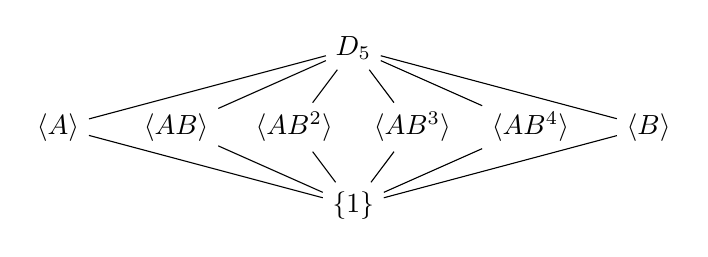
\begin{tikzpicture}
		\node (d5) at (0,2) {$D_5$};
		\node (a) at (-3.75, 1) {$\langle A \rangle$};
		\node (ab) at (-2.25, 1) {$\langle AB \rangle$};
		\node (ab2) at (-0.75, 1) {$\langle AB^2 \rangle$};
		\node (ab3) at (0.75, 1) {$\langle AB^3\rangle$};
		\node (ab4) at (2.25, 1) {$\langle AB^4\rangle$};
		\node (b) at (3.75, 1) {$\langle B \rangle$};
		\node (e) at (0,0) {$\{1\}$};
		
		\draw (e) -- (a)   -- (d5);
		\draw (e) -- (ab)  -- (d5);
		\draw (e) -- (ab2) -- (d5);
		\draw (e) -- (ab3) -- (d5);
		\draw (e) -- (ab4) -- (d5);
		\draw (e) -- (b)   -- (d5);
		\end{tikzpicture}
		\caption{Retículo de subgrupos de $D_5$.}
		\label{ej:reticulod5}
	\end{figure}

	\begin{itemize}
		\item Primera observación. Como $o(B) = 5$ que es primo, tenemos que $o(B^k) = 5,\ k = 1, \dots, 4$. Luego cualquier subgrupo generado por $\langle B^k \rangle = \langle B \rangle$. Aquí falta algo. % TODO revisar este ejemplo que está en la página 85 de santorum
		\item Observemos que los subgrupos propios pueden ser de 2 o 5 elementos.
		\item No puede haber subgrupos generados por dos elementos de $D_5$ (por qué?)
		\item Los únicos subgrupos son $\langle B \rangle$ y los generados por $A, AB, AB^2, AB^3, AB^4$.
		\item Afirmamos que $\{gA\inv{g} \mid g \in G\} = \{\langle A \rangle, \langle AB \rangle, \langle AB^2 \rangle, \langle AB^3 \rangle, \langle AB^4 \rangle \}$. Vamos a probarlo.
		
		\begin{enumerate}
			\item Primero nos damos cuenta de que $\{1, A\} \in N(\langle A \rangle)$.
			\item Además tenemos que no puede haber otro grupo por encima de $\langle A \rangle$ y $D_5$ por lo que tenemos que $N(A) = \langle A \rangle$.
			\item Por tanto en la órbita de $A$ tenemos $[D_5:\langle A \rangle] = 5$ grupos.
		\end{enumerate}
		
	\end{itemize}
\end{ej}
